% Section 3: RL for forecasting (Story 1)
\subsection{RL for forecasting}
\label{sec:rl_for_forecasting}

Section~\ref{sec:bridge} established that a forecaster should be trained
under the decision-induced loss rather than a generic scoring rule. This
section carries that prescription into practice. We call this the
RL-for-forecasting direction, because the object produced is still a
forecaster and reinforcement-learning machinery enters only as the
training method. Three movements organise the section. The single-period
case trains a forecaster against the loss of a single downstream decision
(\S\ref{sec:dfl}). The sequential case carries the same construction
across a horizon, training the forecaster inside an approximate
dynamic-programming loop (\S\ref{sec:adp}). The boundary case
(\S\ref{sec:madeka}) is the most instructive, because it identifies
exactly when the sequential problem is genuinely reinforcement learning
and when it collapses back to supervised learning. That boundary is the
hinge of the chapter, and Sections~\ref{sec:model_based_planning}
and~\ref{sec:forecaster_as_policy} take up the regime on its far side.

\subsubsection{Single-period decision-focused learning}
\label{sec:dfl}

\citet{ElmachtoubGrigas2022} formalise the decision-focused programme for
the class of problems in which the downstream optimisation has a linear
objective. Consider a generic problem in which the decision maker observes
features $x$, forms a forecast $\hat c = f_\theta(x)$ of an unknown cost
vector $c \in \mathbb R^d$, and solves
$z^\star(\hat c) = \arg\min_{z \in \mathcal Z} \hat c^\top z$ over a known
feasible region $\mathcal Z$. A shipping firm picks the cheapest route
through a graph after predicting edge travel times. A portfolio manager
picks asset weights after predicting expected returns. Our newsvendor is
the special case $d = 1$, $\mathcal Z = \mathbb R_+$,
$c = c_o - (c_u + c_o)\, \mathbf 1\{y > a\}$, although the textbook
treatment writes it directly as a quantile problem rather than as a linear
optimisation.

The realised cost of using a predicted $\hat c$ in place of the true $c$
is the suboptimality gap of the induced decision under the true cost,
\begin{equation}
\ell_{\mathrm{SPO}}(\hat c, c)
= c^\top z^\star(\hat c) - \min_{z \in \mathcal Z} c^\top z.
\label{eq:spo_loss}
\end{equation}
This is the SPO loss. It is zero when $z^\star(\hat c) = z^\star(c)$, that
is, when the predicted cost induces the same decision as the true cost,
and is non-negative otherwise. The SPO loss is discontinuous in $\hat c$
because the argmin operator jumps when the predicted cost crosses a face
of $\mathcal Z$, so empirical risk minimisation against $\ell_{\mathrm{SPO}}$
is intractable in general.

\citet{ElmachtoubGrigas2022} derive a convex surrogate via Lagrangian
duality. The SPO$^+$ loss is
\begin{equation}
\ell_{\mathrm{SPO}^+}(\hat c, c)
= \max_{z \in \mathcal Z}\bigl\{ c^\top z - 2 \hat c^\top z \bigr\}
  + 2 \hat c^\top z^\star(c) - \min_{z \in \mathcal Z} c^\top z.
\label{eq:spo_plus_loss}
\end{equation}
The function $\ell_{\mathrm{SPO}^+}$ is convex in $\hat c$, upper-bounds
$\ell_{\mathrm{SPO}}$, and admits the explicit subgradient
$2\bigl(z^\star(c) - z^\star(2 \hat c - c)\bigr) \in
\partial \ell_{\mathrm{SPO}^+}(\hat c, c)$. SPO$^+$ ERM on a linear
hypothesis class reduces to a linear or conic programme and to stochastic
gradient descent for large datasets.

The justification for SPO$^+$ as a stand-in for SPO is Fisher consistency.

\begin{theorem}[\citealp{ElmachtoubGrigas2022}, Theorem 1]
\label{thm:spo_fisher}
Suppose, conditional on $x$, that $\arg\min_{z \in \mathcal Z} \mathbb
E[c \mid x]^\top z$ is a singleton almost surely, that the distribution of
$c \mid x$ is continuous and centrally symmetric about its mean, and that
the interior of $\mathcal Z$ is nonempty. Then any minimiser of the SPO$^+$
population risk over the unrestricted hypothesis class equals the
conditional mean $\mathbb E[c \mid x]$ almost surely, and also minimises
the SPO population risk.
\end{theorem}

The central symmetry assumption is non-trivial. Squared-error regression
is Fisher consistent under the same conditions, so SPO$^+$ and least
squares share the asymptotic-optimality property under
well-specification. The case for SPO$^+$ over least squares is therefore
an argument about finite samples and about robustness to misspecification,
not about asymptotics.\footnote{\citet{LiuGrigas2021} convert Fisher
consistency into a finite-sample calibration bound at rate $n^{-1/4}$ on
polyhedral feasible regions and $n^{-1/2}$ on strongly convex level sets.
\citet{HuKallus2020} show that for contextual linear optimisation under a
margin condition, naive plug-in via least squares attains $n^{-1}$ while
the integrated SPO$^+$ ERM attains only $n^{-2/3}$, so the case for
SPO$^+$ is precisely the misspecified regime. \citet{HuangGupta2024}
construct a perturbation-gradient surrogate whose excess regret is
$\widetilde O((dp/n)^{1/4})$ against the best-in-class policy and remains
valid under misspecification, the modern state of the art. The
\citet{Mandi2024} survey benchmarks eleven DFL techniques on seven
canonical problems and confirms that the empirical advantage of DFL over
predict-then-optimise is largest under misspecification.}

The SPO$^+$ recipe handles linear objectives and convex feasible regions.
\citet{DontiAmosKolter2017} extend the decision-focused programme to
neural-network predictors and to nonlinear stochastic programmes. Given a
parametric forecaster $p(y \mid x; \theta)$ and a downstream optimisation
$z^\star(x; \theta) = \arg\min_z \mathbb E_{y \sim p(y \mid x; \theta)}
[f(x, y, z)]$ subject to convex constraints, they construct the task loss
$L(\theta) = \mathbb E_{(x, y)}[f(x, y, z^\star(x; \theta))]$ and minimise
it by stochastic gradient descent. The technical step is differentiating
the optimal-solution map $z^\star(x; \theta)$ with respect to $\theta$,
which they accomplish by differentiating the Karush-Kuhn-Tucker conditions
of the inner programme and applying the implicit function theorem. The
resulting Jacobian $\partial z^\star / \partial \theta$ flows the gradient
of the task loss back through a learned-prediction layer to the network
weights, and the routine is fast enough at the per-batch level that the
forecaster can be trained end-to-end. On a 24-hour generator-scheduling
task fitted to seven years of PJM electrical-load data,
\citet{DontiAmosKolter2017} report a $38.6\%$ realised-cost reduction
relative to the same Gaussian load model trained on RMSE and plugged into
the same optimisation routine. The implicit-KKT pathway has since become
the standard mechanism for decision-focused training of deep predictors.

The cleanest applied case in the contextual newsvendor family is
\citet{BanRudin2019}. Given $n$ historical observations $(x_i, d_i)$ of
features and realised demand, they solve the single-period newsvendor
loss directly,
\begin{equation}
\hat\beta_n = \arg\min_{\beta \in \mathbb R^p}\frac{1}{n} \sum_{i=1}^n
\Bigl[ c_u (d_i - \beta^\top x_i)^+ + c_o (\beta^\top x_i - d_i)^+ \Bigr]
+ \lambda\, \Omega(\beta),
\label{eq:banrudin_erm}
\end{equation}
with $\Omega$ an $\ell_1$ or $\ell_2$ regulariser. The minimisation
identifies a feature-linear order quantity $q(x) = \hat\beta_n^\top x$
directly, without an intermediate step that estimates a conditional
distribution. Their Theorem 4 derives a finite-sample regret bound that
generalises \citet{Levi2007} to high-dimensional features.\footnote{The bound
scales as $\sqrt{p/n}$ for the $\ell_1$-regularised variant under standard
sub-Gaussian assumptions. A no-feature SAA baseline has a constant $O(1)$
bias that does not shrink in $n$ whenever the conditional mean truly
depends on the features.} On UK hospital emergency-room nurse-staffing
data, the $\ell_1$-regularised ERM saves $23\%$ ($\pounds 44{,}219$ per
ward per year) over a day-of-week-clustered SAA benchmark, and a
kernel-weighted variant attains $24\%$ ($\pounds 46{,}555$). Both
improvements are significant at the $5\%$ level, and the kernel variant
runs in $0.05$ seconds versus the two-orders-of-magnitude slower
benchmark.\footnote{Deep-learning generalisations of the same recipe
parametrise $q(x)$ by a feed-forward network instead of a linear model
\citep{Oroojlooyjadid2020}, and a recent extension uses conditional deep
generative models to handle joint pricing-and-inventory decisions under
decision-dependent uncertainty \citep{HanZhengMisra2024}. The Amazon
Outbound Modeling system \citep{Amazon2025} embeds a probabilistic drain
forecaster as a differentiable simulator inside an off-policy RL ordering
loop, which is the production-scale analogue of the
\citet{DontiAmosKolter2017} task-based training architecture.}

The chapter's thesis line for the single-period case is
\citet{BanRudin2019}'s. ``Rather than a two-step process of first
estimating a demand distribution then optimizing for the optimal order
quantity, we propose solving the Big Data newsvendor problem via
single-step machine learning algorithms.''

\subsubsection{Application: electricity dispatch}
\label{sec:app_electricity}

A microgrid operator must decide how to schedule the next $24$ hours of
electricity generation, energy-storage charging and discharging, and
demand-side flexibility under uncertainty about renewable generation,
load demand, and price. Each scheduling decision $a$ is a vector of
hour-by-hour set-points subject to ramping constraints, state-of-charge
limits, and exchange caps with the main grid. The realised operating
cost depends on which generators were committed and how the realised
renewable output and load tracked the forecast. The downstream problem
is a two-stage robust optimisation. The forecast object is the joint
distribution of renewable output and load demand at $15$-minute
resolution. The application is the cleanest empirical decision-focused
win in the literature because the downstream optimisation has the
linear-plus-convex structure that the SPO machinery above fits exactly.

\citet{CaoXu2025} embed a multilayer probabilistic encoder-decoder
forecaster inside a two-stage robust optimisation solved by the
column-and-constraint generation algorithm. The architecture is a
hierarchy of residual blocks followed by parallel encoder-decoder
chains with a temporal-attention decoder. The training loss combines
the continuous ranked probability score with a regret-type
decision-focused term,
\begin{equation}
\mathrm{Regret}_{\mathrm{SPO}}(y, \hat y)
= J\bigl(\bar z_\rho(\hat y), y\bigr) - J\bigl(z^\star(y), y\bigr),
\label{eq:caoxu_regret}
\end{equation}
where $J(z, y)$ is the realised operating cost of dispatch $z$ under
realisation $y$, $z^\star(y)$ is the oracle dispatch, and
$\bar z_\rho(\hat y)$ is the dispatch produced by a Tikhonov-regularised
convex relaxation of the two-stage robust programme.\footnote{The
downstream problem has binary unit-commitment variables and is therefore
non-differentiable. \citet{CaoXu2025} relax the binaries to $[0, 1]$ and
add $\rho \|z\|^2$ to guarantee strong convexity. Gradients of
\eqref{eq:caoxu_regret} are obtained by implicit differentiation of the
Karush-Kuhn-Tucker residual through the relaxed problem, in the spirit
of \citet{DontiAmosKolter2017}. The forward decision evaluation still
uses the exact mixed-integer programme via column-and-constraint
generation; only the gradient path runs through the convex surrogate.}

Table~\ref{tab:caoxu_breakdown} shows the daily cost breakdown on the
IEEE 33-bus system across four forecasting-optimisation schemes. The
deterministic-forecast pipeline costs \$5{,}127 per day. Replacing the
deterministic forecast with a DeepAR probabilistic forecaster shaves
$5.9\%$. Switching to the \citet{CaoXu2025} encoder-decoder trained on
CRPS shaves $11.5\%$. Adding the decision-focused regret loss to the
encoder-decoder training brings the reduction to $18.0\%$.\footnote{On
the larger 69-bus system the corresponding net-cost reductions are
$4.6\%$, $8.4\%$, and $12.6\%$ from a baseline of \$7{,}521 per day. The
forecasting-only improvements account for roughly two thirds of the
total reduction; the decision-focused fine-tuning contributes the
remaining third. \citet{CaoXu2025} also report a $42\%$ narrowing of
the $95\%$ confidence interval on total operation cost under a
stress-test of the uncertainty budget, which is the calibration
improvement that the SPO programme is theoretically designed to
deliver.}

\begin{table}[h]
\centering
\caption{Daily net operating cost (\$) on the IEEE 33-bus microgrid
for four forecasting-optimisation schemes \citep{CaoXu2025}. The
decision-focused MED-plus-SPO training delivers an $18.0\%$ reduction
over the deterministic baseline.}
\label{tab:caoxu_breakdown}
\begin{tabular}{lcc}
\hline\hline
Scheme              & Net daily cost (\$) & Reduction vs baseline \\
\hline
Deterministic + TSRO      & 5{,}127            & --                  \\
DeepAR + TSRO             & 4{,}823            & $5.9\%$             \\
MED + TSRO (CRPS only)    & 4{,}536            & $11.5\%$            \\
MED + SPO + TSRO          & 4{,}205            & $18.0\%$            \\
\hline\hline
\end{tabular}
\end{table}

The forecast-side gains and the decision-side gains decompose cleanly.
The encoder-decoder's CRPS reduction over DeepAR captures
forecast-accuracy improvements that the operator could in principle
have obtained without changing the optimisation routine. The
MED-plus-SPO fine-tuning captures a further decision-aware adjustment
that does not improve the CRPS but does improve realised operating
cost. The chapter's thesis statement carries over directly. The
proposed method aligns forecasting accuracy with operational objectives
by directly minimising decision regret via a surrogate SPO loss. The
\citet{DontiAmosKolter2017} PJM result of $38.6\%$ cost reduction at
the larger-scale grid level reaches the same qualitative conclusion.

\subsubsection{Simulation: decision-focused forecasting under AR(1) demand}
\label{sec:forecasting_rl_sim}

A clean synthetic instance makes the decision-focused claim concrete on
a substrate that an econometrician would recognise. The DGP is the
contextual AR(1) demand
\begin{equation}
y_t = \mu + \phi (y_{t-1} - \mu) + \beta^\top x_t + \sigma_t\,
\varepsilon_t, \qquad \varepsilon_t \sim \mathcal N(0, 1),
\label{eq:ar1_dgp}
\end{equation}
with $x_t \in \mathbb R^{10}$ drawn i.i.d.\ standard normal, persistence
$\phi = 0.7$, demand mean $\mu = 10$, and a heteroscedastic noise
scale $\sigma_t = \sigma_0 \exp(\gamma^\top x_t)$ with $\sigma_0 = 1$
and a per-seed $\gamma$. The hypothesis class assumes homoscedasticity,
so the heteroscedasticity is the misspecification axis. The newsvendor
cost parameters of Section~\ref{sec:forecasting_rl_intro} carry over.
$c_u = 4$, $c_o = 1$, $\tau^\star = 0.8$. Each procedure trains on
$T = 2{,}000$ in-sample periods and evaluates on $500$ out-of-sample
periods, averaged over $20$ paired random seeds.

Three procedures share the AR(1)-plus-linear hypothesis class.
\emph{Method A} fits $(\mu, \phi, \beta, \sigma)$ by ordinary least
squares and plugs the fitted Gaussian distribution into the critical
fractile, $q^{\mathrm A}_t = \hat\mu + \hat\phi (y_{t-1} - \hat\mu) +
\hat\beta^\top x_t + \hat\sigma\, \Phi^{-1}(\tau^\star)$. This is the
classical estimate-then-optimise pipeline. \emph{Method B} trains the
same parametric family by direct subgradient descent on the realised
newsvendor loss, the decision-focused-learning approach of
\citet{DontiAmosKolter2017}, and uses the same plug-in formula at
decision time. \emph{Method
C} takes the OLS mean prediction and replaces the parametric residual
quantile $\hat\sigma\, \Phi^{-1}(\tau^\star)$ with the empirical
residual quantile, the simplest one-step rollout in the spirit of
\citet{BertsekasRollout2022}.

\begin{table}[h]
\centering
\caption{Decision-focused forecasting under AR(1) demand with
heteroscedastic noise, $20$ seeds, standard errors in parentheses.
Method B attains the same in-sample MSE as Method A but a factor-of-five
lower realised newsvendor regret.}
\label{tab:forecasting_rl_sim}
% Generated by decision_focused_ar1.py
\begin{tabular}{lccc}
\hline\hline
Method & In-sample MSE & Out-of-sample MSE & Mean newsvendor regret \\
\hline
A: OLS + critical fractile & $44.913\,(18.696)$ & $530.014\,(498.341)$ & $2.819\,(0.670)$ \\
B: Task-loss fine-tune & $45.646\,(18.789)$ & $529.350\,(497.261)$ & $0.597\,(0.142)$ \\
C: Bertsekas rollout & $44.913\,(18.696)$ & $530.014\,(498.341)$ & $0.946\,(0.177)$ \\
\hline\hline
\end{tabular}

\end{table}

\begin{figure}[h]
\centering
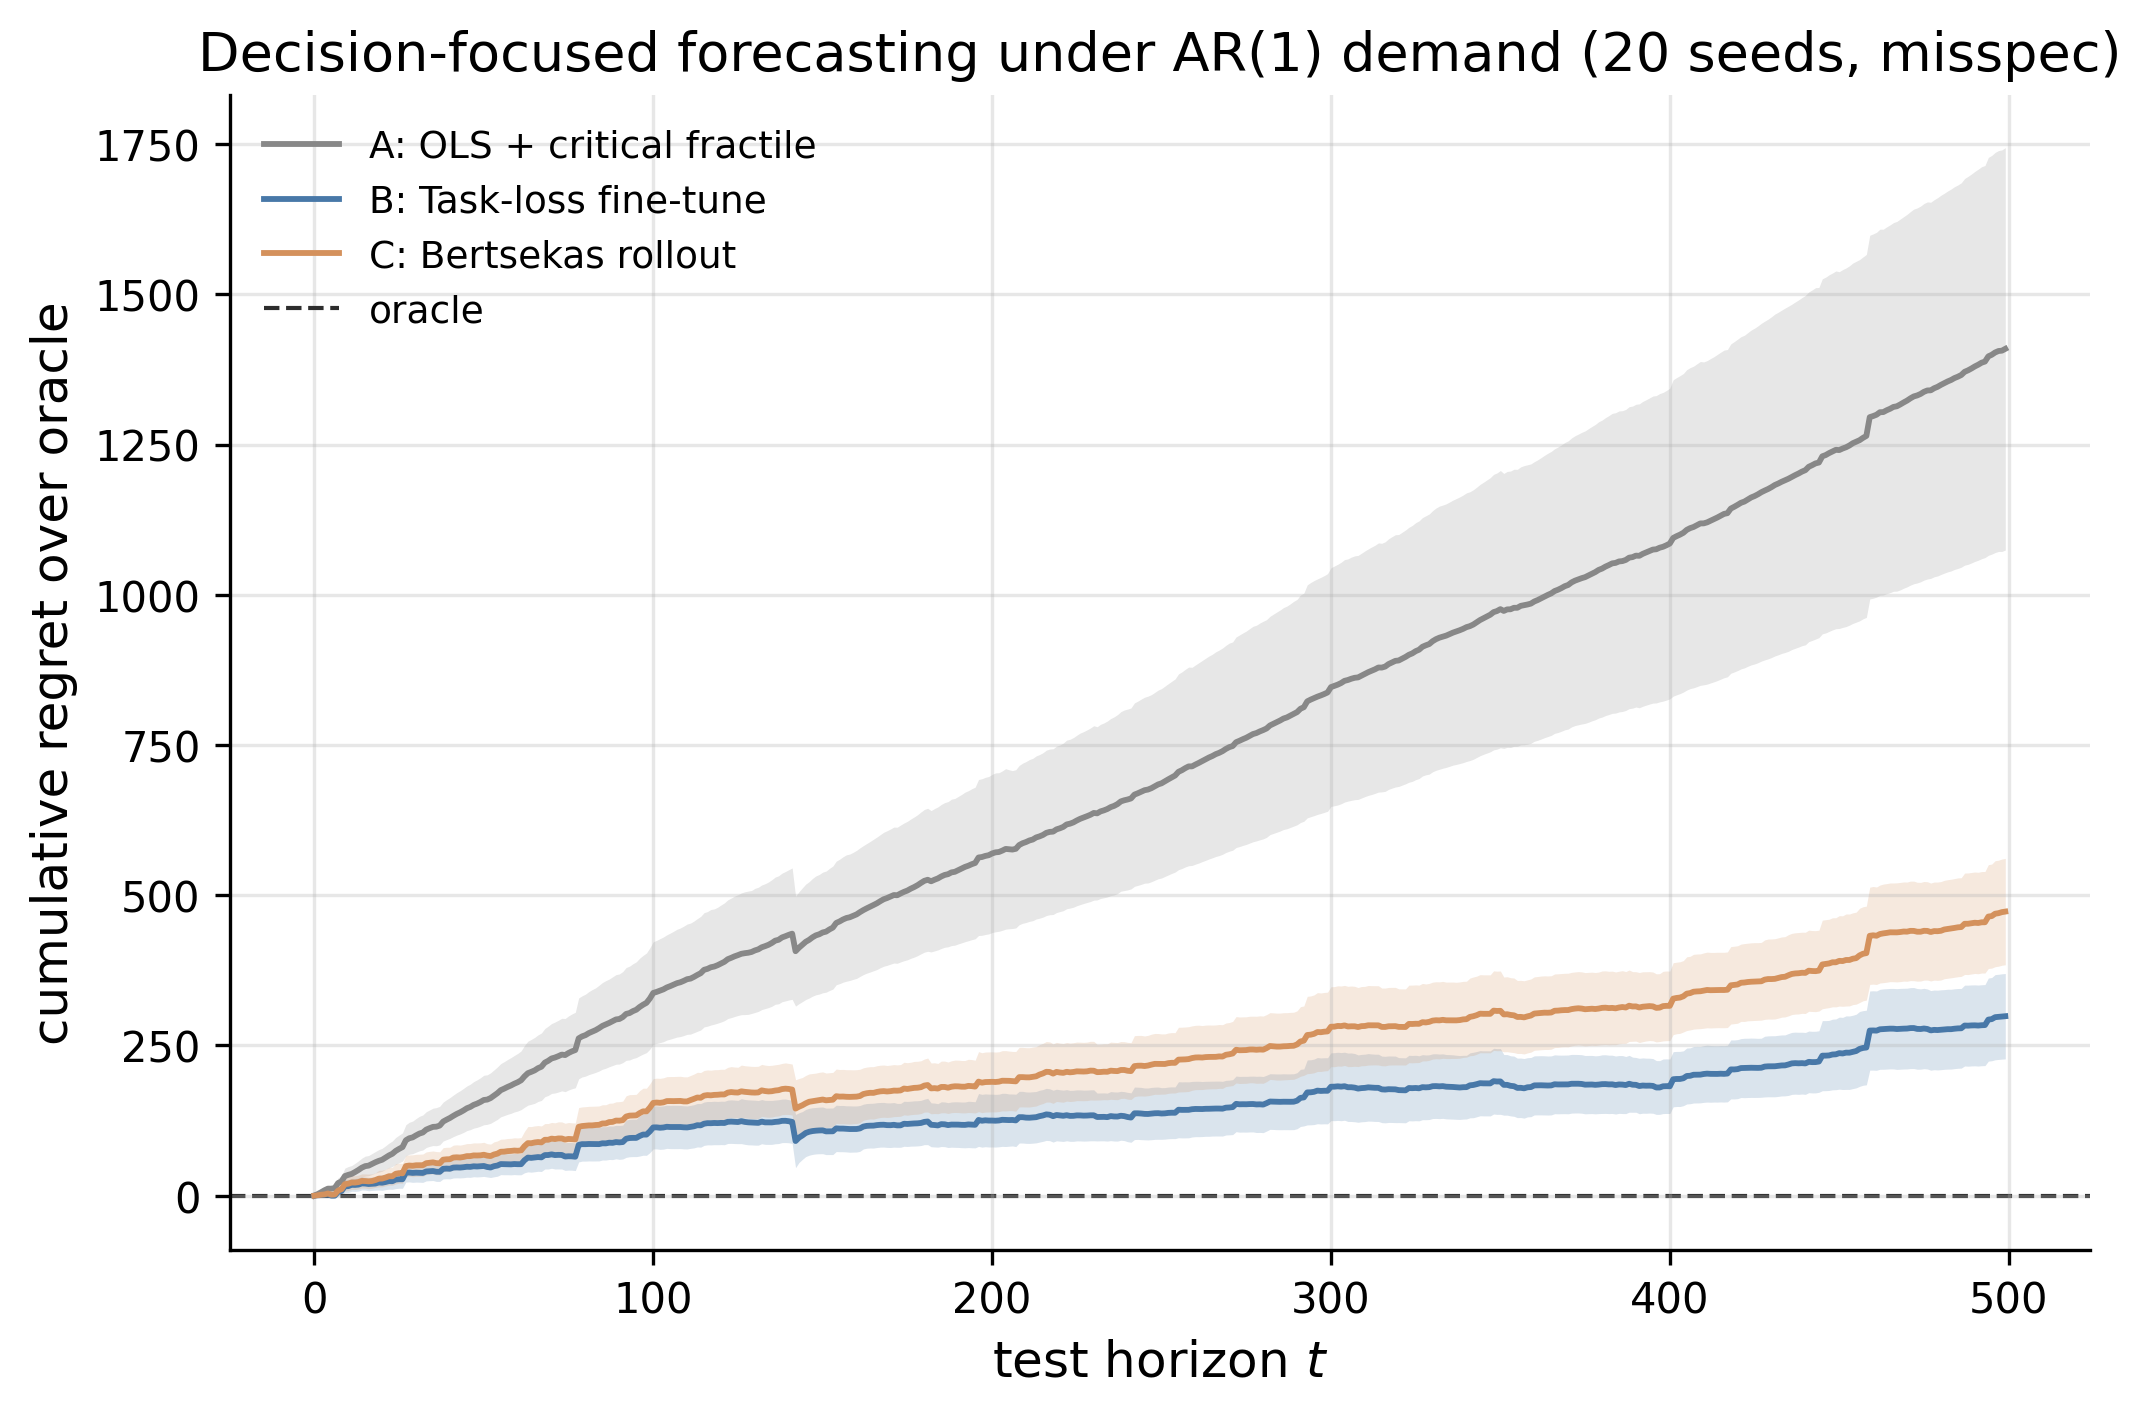
\includegraphics[width=0.85\linewidth]{../ch12_forecasting_rl/sims/decision_focused_ar1.png}
\caption{Cumulative newsvendor regret over the test horizon, $20$
seeds. The shaded band is one standard error of the mean. The
horizontal line at zero is the oracle. Method B (SPO$^+$ fine-tune)
attains the lowest regret; Method A (OLS plus critical fractile) the
highest.}
\label{fig:forecasting_rl_sim}
\end{figure}

Table~\ref{tab:forecasting_rl_sim} reports the realised costs. Method
A's in-sample MSE is $44.91 \pm 18.70$ and Method B's is $45.65 \pm
18.79$, statistically indistinguishable. Method C inherits Method A's
MSE by construction. The MSE ranking declares the three forecasters
equivalent. The realised newsvendor regret over $500$ test periods
diverges sharply. Method A attains $2.82 \pm 0.67$, Method B attains
$0.60 \pm 0.14$, and Method C attains $0.95 \pm 0.18$. Method B's
regret is a factor of $4.7$ lower than Method A's, and Method C's is a
factor of $3.0$ lower, both with standard errors that exclude zero.
Figure~\ref{fig:forecasting_rl_sim} plots the cumulative regret over
the test horizon.

The pattern is the Granger-Pesaran phenomenon of Section~\ref{sec:bridge}
on a familiar substrate. The MSE ranking and the decision-induced
ranking disagree once the noise model is misspecified, and a forecaster
that trades off in-sample squared error for in-sample realised cost
wins on realised cost out of sample. The simulation is also a worked
example of the \citet{HuKallus2020} counterpoint. Under
well-specification with $\gamma = 0$ the three methods are
indistinguishable on regret as well as on MSE, so the case for
decision-focused training and rollout is conditional on the
heteroscedasticity that the homoscedastic OLS model cannot represent.
The remainder of this section asks what changes when the decision is
sequential rather than one-shot.

\subsubsection{Sequential: approximate dynamic programming for forecasters}
\label{sec:adp}

The single-period newsvendor of \S\ref{sec:dfl} becomes a sequential
problem the moment the retailer carries inventory between periods. Today's
order $a_t$ affects tomorrow's starting state $s_{t+1}$, and the
realised cost $L(a_t, y_t)$ aggregates into a discounted return
$\sum_{t \ge 0} \gamma^t L(a_t, y_t)$. The standard dynamic programming
recursion gives the optimal policy via the Bellman equation
$V^\star(s) = \min_a \{ \mathbb E_y[L(a, y) + \gamma V^\star(s')]\}$, with
$s'$ the next state. The exact recursion is intractable whenever the
state space is high-dimensional or the next-state transition is unknown,
which is the regime that motivates approximate dynamic programming and
its modern reinforcement-learning descendants.

\citet{BertsekasRollout2022} provides the unifying frame for ADP applied
to sequential estimation. A measurement policy at time $k$ is a function
from the current posterior $b_k$ over an unknown parameter $\theta$ to
the next observation point $u_{k+1}$, and the exact dynamic programming
recursion
\begin{equation}
J^\star_k(b_k) = \min_{u_{k+1}}\Bigl\{
  c(u_{k+1}) + \mathbb E_{z_{u_{k+1}}}\bigl[
    J^\star_{k+1}\bigl(B_k(b_k, u_{k+1}, z_{u_{k+1}})\bigr)
  \bigr] \Bigr\}
\label{eq:bertsekas_dp}
\end{equation}
is infeasible because the posterior space is infinite-dimensional. The
rollout approximation replaces the unknown optimal continuation
$J^\star_{k+1}$ with the cost-to-go of a base policy
$\widetilde J_{k+1}$ that can be evaluated by Monte Carlo simulation. The
cost-improvement guarantee, namely that the rollout policy weakly
dominates the base policy under a mild contractivity condition, is the
formal underpinning of the entire programme. Certainty equivalence
further reduces the Monte Carlo burden by replacing the stochastic
continuation cost with its expectation conditional on the realised first
step. The same vocabulary covers Bayesian optimisation, sequential decoding,
and adaptive Bayesian experiment design.

\citet{Fernandes2024} applies the neuro-dynamic-programming variant of this
machinery to quarterly gross domestic product nowcasting. The Bellman
equation is
\begin{equation}
J(i) = \min_u \mathbb E\bigl[ g(i, u, j) + \alpha\, J(j) \bigr],
\label{eq:fernandes_bellman}
\end{equation}
where $i$ is the current state of the economy (regularised levels of
industrial production, construction output, retail trade turnover, goods
exports, goods imports, and the European Commission's Economic Sentiment
Indicator), $u$ is the quarter-over-quarter change of output, the cost
$g(i, u, j) = u^2$ is a quadratic adjustment cost in the spirit of
Lucas-Prescott (1971), and $\alpha \in (0, 1)$ is the discount factor. The
reward signal is not the cross-sectional forecast error of OLS. It is the
temporal difference between successive predictions of the GDP level. The
value function $J^\star$ is approximated by a single-hidden-layer
feed-forward network and trained by Sutton's temporal-difference algorithm.

\begin{algorithm}[h]
\caption{TD(0) with neural cost-to-go approximation \citep{Fernandes2024}}
\label{alg:fernandes_td0}
\begin{algorithmic}[1]
\State $\delta \gets \widetilde J(i, r) - \alpha \widetilde J(j, r) - g(i, u, j)$
\State $r_k \gets r_k - \gamma\, \delta\, h_k(i)$
  \Comment{output-layer update}
\State $r_{k\ell} \gets r_{k\ell} - \gamma\, \delta\, r_k\,
  \nabla_{r_{k\ell}} h_k(i)$
  \Comment{hidden-layer update}
\State \Return $r$
\end{algorithmic}
\end{algorithm}

Training uses a panel of $26$ European Union countries with $2{,}470$
quarterly transitions across $2000$Q1 to $2023$Q4, with Portugal held out
for evaluation over $2015$Q1 to $2023$Q4. Two findings matter for the
chapter. On the regularised Portuguese GDP level, the OLS benchmark
fitted on Portugal-only data attains a mean absolute error of $6.61\%$ of
the range and a root mean squared error of $8.32\%$. The TD-trained
neural network on the EU-ex-Portugal panel attains $4.53\%$ MAE and
$5.97\%$ RMSE, a $32\%$ reduction in MAE and a $28\%$ reduction in RMSE
relative to OLS. A linear architecture trained with the same TD algorithm
on the same panel attains only $10.70\%$ MAE, which establishes that the
gain is attributable to the nonlinear approximation and not to the
panel-data augmentation alone. The second finding is methodological. The
panel-data training transfers cleanly to the held-out country, which
alleviates the small-$T$ problem that plagues macroeconomic forecasting
and is the most concrete macro-domain validation of NDP on record.

A distinct strand uses reinforcement learning not as the forecaster
directly but as a meta-algorithm that adapts ensemble weights over a
portfolio of base forecasters \citep{Fu2022}. The state is the recent
window of the time series plus a log of per-model performance, the
action is a vector of non-negative weights on the simplex, and the
reward is the negative one-step forecast error. The methodological
contribution is modest. The model-combination problem is also an online
learning problem, and Hedge or EXP3 attains the same $O(\sqrt{T \log N})$
regret rate against the best fixed combination in hindsight. We mention
this strand for scope and move on.

\subsubsection{The boundary: deep inventory management}
\label{sec:madeka}

The sequential constructions of \S\ref{sec:adp} still produce a
forecaster as their artifact. Their most developed industrial instance is
the deep inventory-management system of \citet{Madeka2022DeepInventory},
who treat periodic-review inventory control with stochastic vendor lead
times, lost sales, correlated demand, and price matching as a sequential
decision problem whose forecast object is the joint distribution of
demand and lead time over a finite horizon. The technical device is
DirectBackprop, a differentiable historical-data simulator that lets
policy gradients flow through the realised inventory cost while the
exogenous processes are resampled from history. A learned ordering policy
parametrised by a deep network beats classical newsvendor and model-free
reinforcement-learning baselines on more than $10{,}000$ Amazon SKUs,
which makes it the direct multi-period generalisation of the
\citet{BanRudin2019} single-period empirical risk minimisation.

The reason this is the boundary of the RL-for-forecasting direction,
rather than a member of it, is a reduction theorem.
\citet{Madeka2022DeepInventory} prove that for the exogenous-decision-process
subclass, in which the dynamics depend on exogenous shocks but the agent's
actions do not feed back into demand or lead time, the
reinforcement-learning problem reduces to supervised learning against the
realised cost.\footnote{The reduction recovers the $\sqrt{p/n}$ regret
rate of \citet{BanRudin2019} as a special case and supplies a
finite-sample bound for the sequential version.} When that condition
holds, the sequential problem is decision-focused supervised learning
carried across a horizon, and the word reinforcement is ceremonial. When
the condition fails, that is, when the agent's actions move the
distribution of future demand or prices, the reduction breaks and the
problem is genuinely reinforcement learning. That distinction is the
hinge of the chapter. Sections~\ref{sec:model_based_planning}
and~\ref{sec:forecaster_as_policy} take up the regime on the far side of
it, where the forecaster is no longer the artifact but a component inside
the agent.
